\documentclass[11pt,a4paper]{article}

% Packages
\usepackage[utf8]{inputenc}
\usepackage[T1]{fontenc}
\usepackage{amsmath,amssymb,amsfonts}
\usepackage{graphicx}
\usepackage{booktabs}
\usepackage{multirow}
\usepackage{xcolor}
\usepackage{hyperref}
\usepackage{algorithm}
\usepackage{algpseudocode}
\usepackage{listings}
\usepackage{tikz}
\usetikzlibrary{shapes,arrows,positioning,fit,backgrounds}
\usepackage[margin=1in]{geometry}
\usepackage{natbib}
\usepackage{subcaption}
\usepackage{float}

% Custom colors
\definecolor{botred}{RGB}{231,76,60}
\definecolor{hubblue}{RGB}{52,152,219}
\definecolor{organicgreen}{RGB}{46,204,113}
\definecolor{automatedorange}{RGB}{230,126,34}

% Code listing style
\lstset{
    basicstyle=\ttfamily\small,
    breaklines=true,
    frame=single,
    backgroundcolor=\color{gray!10},
    keywordstyle=\color{blue},
    commentstyle=\color{green!60!black},
    stringstyle=\color{red!60!black}
}

% Title
\title{\textbf{LogGhostbuster: A Hybrid Machine Learning System for Bot Detection and Download Pattern Classification in Scientific Repository Logs}}

\author{
    Yasset Perez-Riverol$^{1,*}$\\
    \small $^{1}$European Molecular Biology Laboratory, European Bioinformatics Institute (EMBL-EBI),\\
    \small Wellcome Genome Campus, Hinxton, Cambridge CB10 1SD, UK\\
    \small $^{*}$Corresponding author: yperez@ebi.ac.uk
}

\date{}

\begin{document}

\maketitle

% Abstract
\begin{abstract}
\textbf{Motivation:} Scientific data repositories face increasing challenges from automated bot traffic that inflates download statistics, affects resource allocation decisions, and obscures genuine usage patterns. Distinguishing between legitimate automated access (mirrors, CI/CD pipelines) and malicious bots (scrapers, crawlers) requires sophisticated analysis of behavioral patterns that simple rule-based systems cannot capture.

\textbf{Results:} We present LogGhostbuster, a hybrid machine learning system that combines unsupervised anomaly detection with hierarchical classification to identify bot behavior in download logs. The system implements a three-level taxonomy distinguishing organic (human) from automated behavior, and further classifying automated access as either malicious bots or legitimate automation. Using Isolation Forest for anomaly detection and an optional Transformer-based deep architecture for temporal pattern recognition, LogGhostbuster achieves robust classification with configurable rules and provider-agnostic design. Applied to the PRIDE database at EMBL-EBI, the system identified 20,903 bot locations (29.4\% of 71,133 analyzed) responsible for 113.1 million downloads (71.0\% of total), while correctly distinguishing 667 legitimate automation sources including institutional mirrors.

\textbf{Availability:} LogGhostbuster is freely available at \url{https://github.com/bigbio/logghostbuster} under the Apache 2.0 license.

\textbf{Keywords:} bot detection, machine learning, anomaly detection, download statistics, scientific repositories
\end{abstract}

\section{Introduction}

Scientific data repositories have become essential infrastructure for research, hosting petabytes of data accessed by millions of users worldwide \citep{Perez2019}. Repositories such as the PRIDE database \citep{Perez-Riverol2022}, the European Nucleotide Archive (ENA) \citep{Leinonen2011}, and UniProt \citep{UniProtConsortium2023} provide critical resources for the scientific community. Understanding how these resources are used is essential for resource allocation, impact assessment, and service improvement.

However, download statistics from scientific repositories are increasingly contaminated by automated bot traffic. Studies have shown that bot traffic can account for 30-70\% of web requests \citep{Imperva2023}, with scientific repositories being particularly attractive targets due to their open access policies and valuable data content. This contamination creates several problems:

\begin{enumerate}
    \item \textbf{Inflated metrics}: Download counts used for impact assessment become unreliable when dominated by automated access.
    \item \textbf{Resource misallocation}: Infrastructure decisions based on apparent demand may not reflect actual user needs.
    \item \textbf{Obscured patterns}: Genuine usage trends become difficult to identify amid bot noise.
    \item \textbf{Service degradation}: High-volume automated access can degrade service quality for human users.
\end{enumerate}

Distinguishing bot traffic from human access is challenging because not all automated access is problematic. Legitimate automation includes institutional mirrors that improve global access, continuous integration pipelines that test software against repository data, and data aggregation services that provide valuable meta-analyses. A successful bot detection system must therefore implement a nuanced classification that distinguishes malicious from legitimate automation.

Existing approaches to bot detection typically fall into two categories: signature-based methods that identify known bot user agents and IP ranges, and behavioral analysis that identifies bot-like access patterns \citep{Jonker2019}. Signature-based methods suffer from easy circumvention through user agent spoofing, while simple behavioral rules miss sophisticated bots that mimic human patterns. Machine learning approaches have shown promise \citep{Rovetta2020}, but most focus on web security rather than scientific repository contexts where different patterns prevail.

In this paper, we present LogGhostbuster, a hybrid machine learning system specifically designed for bot detection in scientific repository download logs. Our contributions include:

\begin{itemize}
    \item A \textbf{hierarchical classification taxonomy} that distinguishes organic (human-like) from automated behavior, and further classifies automated access as malicious bots or legitimate automation.
    \item A \textbf{hybrid detection architecture} combining Isolation Forest anomaly detection with rule-based and optional deep learning classification.
    \item A \textbf{provider-agnostic design} that supports different log formats through configurable schema mappings and extensible feature extraction.
    \item \textbf{Comprehensive evaluation} on real-world data from the PRIDE proteomics database, demonstrating the system's effectiveness in a production environment.
\end{itemize}

\section{Background}

\subsection{Bot Detection Challenges}

Bot detection in web traffic has been extensively studied in the security community \citep{Iliou2021}. Traditional approaches include:

\textbf{Signature-based detection} relies on matching known bot signatures such as user agent strings, IP address ranges, or access patterns. While effective against unsophisticated bots, these methods fail against bots that spoof legitimate user agents or use residential proxies \citep{Jonker2019}.

\textbf{Behavioral analysis} examines access patterns to identify non-human behavior. Metrics such as request rate, session duration, and navigation patterns can distinguish bots from humans \citep{Rovetta2020}. However, sophisticated bots increasingly mimic human behavior, reducing the effectiveness of simple rules.

\textbf{Machine learning approaches} have shown promise in capturing complex patterns that simple rules miss. Both supervised \citep{Cabri2021} and unsupervised \citep{Habibi2020} methods have been applied, with ensemble approaches often achieving the best results.

\subsection{Scientific Repository Context}

Bot detection in scientific repositories presents unique challenges:

\begin{enumerate}
    \item \textbf{Legitimate automation}: Unlike e-commerce sites where automation is generally unwanted, scientific repositories benefit from mirrors, aggregators, and automated pipelines.
    \item \textbf{Download-centric patterns}: Scientific repositories primarily serve file downloads rather than page views, requiring different feature engineering.
    \item \textbf{Long-term patterns}: Bot campaigns against repositories may span months or years, requiring temporal analysis across extended periods.
    \item \textbf{Geographic distribution}: Global scientific collaboration means legitimate access comes from diverse locations, making geographic filtering problematic.
\end{enumerate}

\subsection{Isolation Forest}

Isolation Forest \citep{Liu2008} is an unsupervised anomaly detection algorithm particularly suited to high-dimensional data. Unlike distance-based methods, Isolation Forest identifies anomalies by their susceptibility to isolation through random partitioning.

The algorithm constructs an ensemble of isolation trees, each built by recursively partitioning the data using random feature selections and split points. Anomalies, being rare and different, require fewer partitions to isolate and thus have shorter average path lengths in the trees.

For a data point $x$, the anomaly score is computed as:
\begin{equation}
    s(x, n) = 2^{-\frac{E(h(x))}{c(n)}}
\end{equation}
where $E(h(x))$ is the expected path length of $x$ across all trees, $n$ is the sample size, and $c(n)$ is a normalization factor.

Isolation Forest has several advantages for our application:
\begin{itemize}
    \item No assumption about the distribution of normal data
    \item Linear time complexity O($n \log n$)
    \item Effective in high-dimensional spaces
    \item Robust to irrelevant features
\end{itemize}

\section{Methods}

\subsection{System Architecture}

LogGhostbuster implements a multi-stage pipeline (Figure~\ref{fig:architecture}) comprising:

\begin{enumerate}
    \item \textbf{Data Ingestion}: Memory-efficient loading and optional sampling of Parquet files via DuckDB.
    \item \textbf{Feature Extraction}: Computation of 60+ behavioral features at the location (IP/geo) level.
    \item \textbf{Anomaly Detection}: Isolation Forest identifies statistically unusual access patterns.
    \item \textbf{Classification}: Hierarchical classification using rules or deep learning.
    \item \textbf{Reporting}: Generation of annotated data and comprehensive reports.
\end{enumerate}

\begin{figure}[H]
\centering
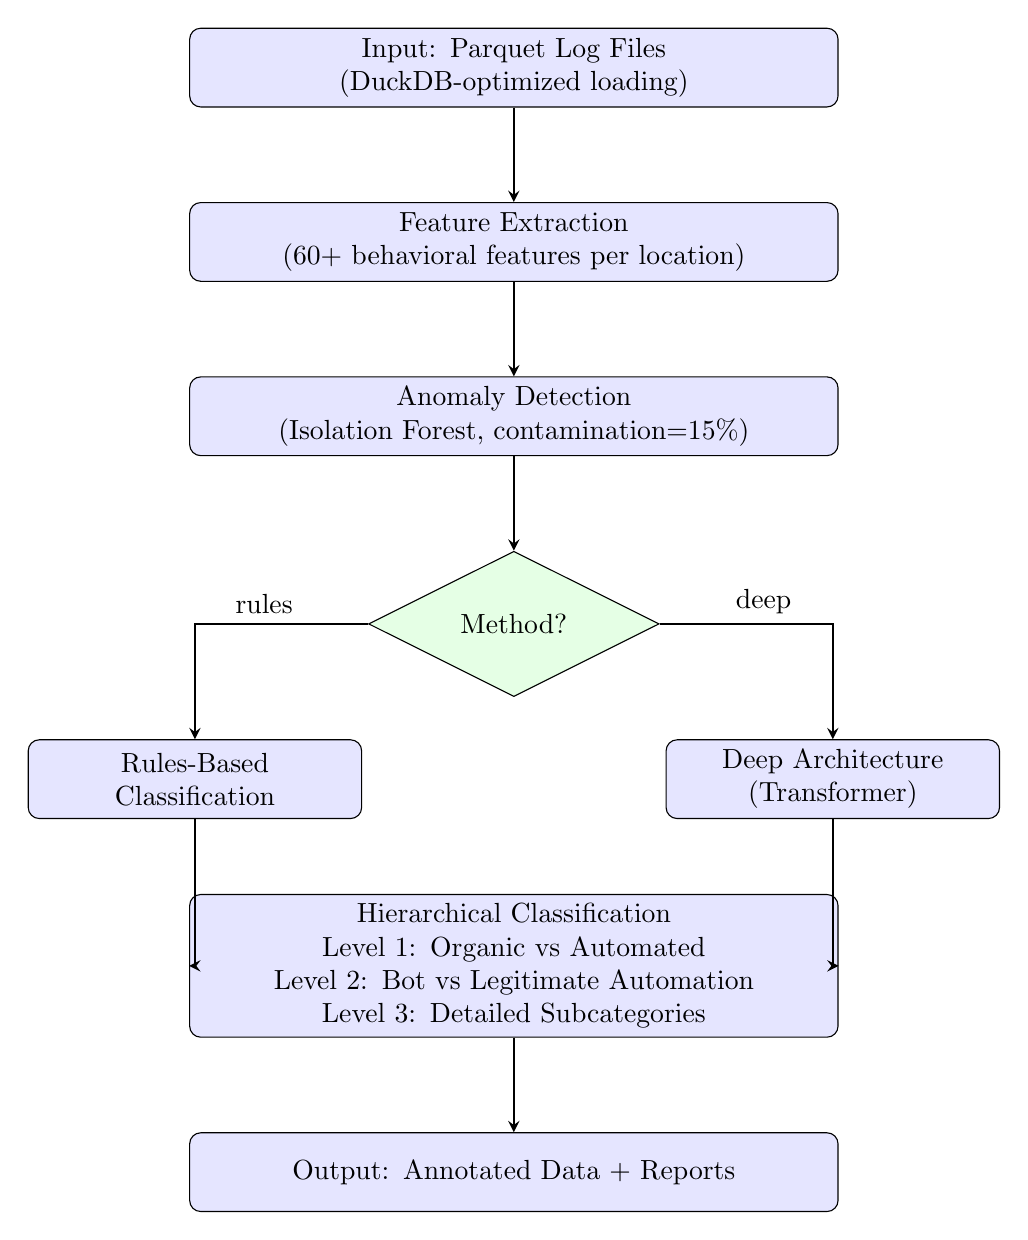
\begin{tikzpicture}[
    node distance=1.2cm,
    block/.style={rectangle, draw, fill=blue!10, text width=8cm, text centered, rounded corners, minimum height=1cm},
    decision/.style={diamond, draw, fill=green!10, text width=2.5cm, text centered, aspect=2},
    arrow/.style={->, >=stealth, thick}
]

% Nodes
\node[block] (input) {Input: Parquet Log Files\\(DuckDB-optimized loading)};
\node[block, below=of input] (features) {Feature Extraction\\(60+ behavioral features per location)};
\node[block, below=of features] (anomaly) {Anomaly Detection\\(Isolation Forest, contamination=15\%)};
\node[decision, below=of anomaly] (method) {Method?};
\node[block, below left=1cm and 1cm of method, text width=4cm] (rules) {Rules-Based\\Classification};
\node[block, below right=1cm and 1cm of method, text width=4cm] (deep) {Deep Architecture\\(Transformer)};
\node[block, below=2.5cm of method] (hier) {Hierarchical Classification\\Level 1: Organic vs Automated\\Level 2: Bot vs Legitimate Automation\\Level 3: Detailed Subcategories};
\node[block, below=of hier] (output) {Output: Annotated Data + Reports};

% Arrows
\draw[arrow] (input) -- (features);
\draw[arrow] (features) -- (anomaly);
\draw[arrow] (anomaly) -- (method);
\draw[arrow] (method) -| node[above, pos=0.3] {rules} (rules);
\draw[arrow] (method) -| node[above, pos=0.3] {deep} (deep);
\draw[arrow] (rules) |- (hier);
\draw[arrow] (deep) |- (hier);
\draw[arrow] (hier) -- (output);

\end{tikzpicture}
\caption{LogGhostbuster system architecture showing the multi-stage pipeline from data ingestion through classification and reporting.}
\label{fig:architecture}
\end{figure}

\subsection{Feature Extraction}

Features are computed at the \textit{location} level, where a location represents a unique geographic origin (typically derived from IP geolocation). This aggregation reduces millions of individual download events to thousands of location profiles, making analysis tractable while preserving behavioral patterns.

\subsubsection{Basic Activity Features}

\begin{itemize}
    \item \texttt{unique\_users}: Number of distinct user identifiers from this location
    \item \texttt{downloads\_per\_user}: Ratio of total downloads to unique users
    \item \texttt{total\_downloads}: Aggregate download count
    \item \texttt{projects\_per\_user}: Diversity of accessed resources
\end{itemize}

\subsubsection{Temporal Features}

Temporal patterns are critical for bot detection, as automated access often exhibits characteristic timing signatures:

\begin{itemize}
    \item \texttt{hourly\_entropy}: Shannon entropy of hourly download distribution. Bots often show low entropy (concentrated activity) while humans show higher entropy (distributed activity).
    \item \texttt{working\_hours\_ratio}: Fraction of downloads during business hours (9 AM - 6 PM local time). Human users typically show higher ratios.
    \item \texttt{night\_activity\_ratio}: Fraction of downloads during night hours. Elevated night activity suggests automated scheduling.
    \item \texttt{yearly\_entropy}: Distribution of activity across years, detecting sudden spikes.
    \item \texttt{spike\_ratio}: Ratio of latest year downloads to historical average.
\end{itemize}

\subsubsection{Behavioral Features (Deep Method)}

Advanced features capture nuanced behavioral patterns:

\begin{itemize}
    \item \texttt{burst\_pattern\_score}: Detects concentrated download bursts within short time windows.
    \item \texttt{circadian\_rhythm\_deviation}: Measures deviation from typical human circadian patterns.
    \item \texttt{user\_coordination\_score}: Identifies synchronized activity across multiple user IDs, suggesting bot farms.
    \item \texttt{regularity\_score}: Measures temporal regularity, with high values indicating scheduled automation.
\end{itemize}

\subsubsection{Discriminative Features}

Features designed to distinguish malicious bots from legitimate automation:

\begin{itemize}
    \item \texttt{file\_exploration\_score}: Breadth of file access (bots often scrape systematically)
    \item \texttt{file\_mirroring\_score}: Pattern consistency with mirroring behavior
    \item \texttt{bot\_farm\_score}: User homogeneity suggesting coordinated fake accounts
    \item \texttt{geographic\_stability}: IP diversity from this location
    \item \texttt{legitimate\_automation\_score}: Composite score for legitimate automation indicators
\end{itemize}

\subsection{Hierarchical Classification Taxonomy}

LogGhostbuster implements a three-level classification taxonomy (Figure~\ref{fig:taxonomy}):

\begin{figure}[H]
\centering
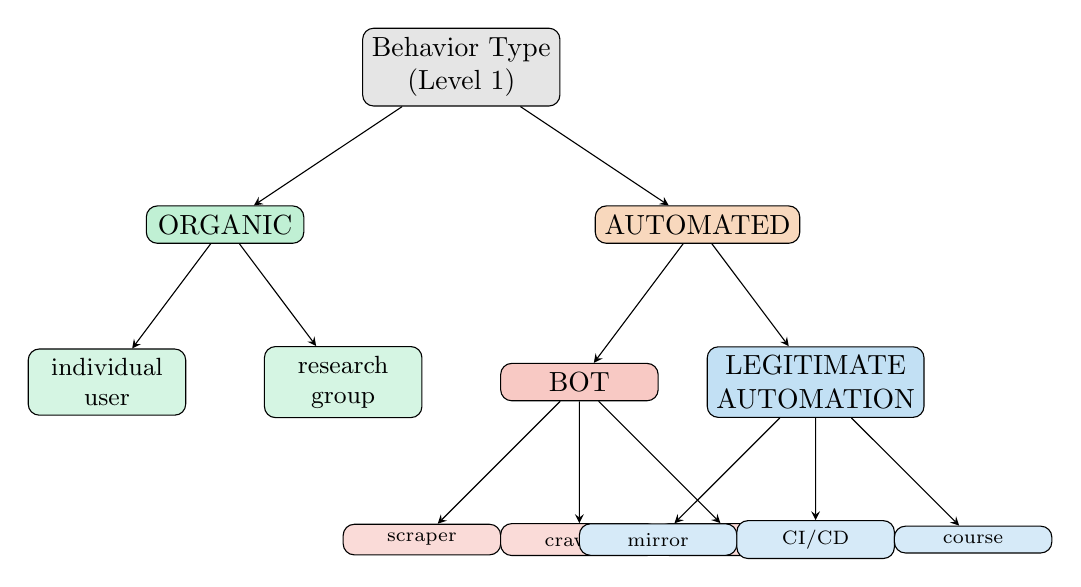
\begin{tikzpicture}[
    level 1/.style={sibling distance=6cm, level distance=2cm},
    level 2/.style={sibling distance=3cm, level distance=2cm},
    level 3/.style={sibling distance=2cm, level distance=2cm},
    every node/.style={draw, rounded corners, align=center, minimum width=2cm},
    edge from parent/.style={draw, ->, >=stealth}
]

\node[fill=gray!20] {Behavior Type\\(Level 1)}
    child {node[fill=organicgreen!30] {ORGANIC}
        child {node[fill=organicgreen!20, font=\small] {individual\\user}}
        child {node[fill=organicgreen!20, font=\small] {research\\group}}
    }
    child {node[fill=automatedorange!30] {AUTOMATED}
        child {node[fill=botred!30] {BOT}
            child {node[fill=botred!20, font=\scriptsize] {scraper}}
            child {node[fill=botred!20, font=\scriptsize] {crawler}}
            child {node[fill=botred!20, font=\scriptsize] {coordinated}}
        }
        child {node[fill=hubblue!30] {LEGITIMATE\\AUTOMATION}
            child {node[fill=hubblue!20, font=\scriptsize] {mirror}}
            child {node[fill=hubblue!20, font=\scriptsize] {CI/CD}}
            child {node[fill=hubblue!20, font=\scriptsize] {course}}
        }
    };

\end{tikzpicture}
\caption{Three-level hierarchical classification taxonomy. Level 1 distinguishes organic (human-like) from automated behavior. Level 2 classifies automated behavior as malicious bot or legitimate automation. Level 3 provides detailed subcategories.}
\label{fig:taxonomy}
\end{figure}

\subsubsection{Level 1: Behavior Type}

The first level distinguishes fundamental behavior patterns:

\textbf{ORGANIC}: Human-like download patterns characterized by:
\begin{itemize}
    \item Working hours activity ($\texttt{working\_hours\_ratio} \geq 0.4$)
    \item Low regularity ($\texttt{regularity\_score} \leq 0.6$)
    \item Irregular temporal distribution ($\texttt{interval\_cv} \geq 0.7$)
    \item Limited user counts (typically $< 50$ unique users)
\end{itemize}

\textbf{AUTOMATED}: Programmatic access patterns characterized by:
\begin{itemize}
    \item High regularity ($\texttt{regularity\_score} \geq 0.7$)
    \item Non-working hours activity ($\texttt{night\_activity\_ratio} \geq 0.35$)
    \item User coordination ($\texttt{user\_coordination\_score} \geq 0.6$)
    \item Very high download rates ($\texttt{downloads\_per\_user} \geq 500$)
\end{itemize}

\subsubsection{Level 2: Automation Category}

Within automated behavior, the second level distinguishes intent:

\textbf{BOT} (Malicious automation):
\begin{itemize}
    \item Many users with low downloads per user (bot farms)
    \item High coordination across user IDs
    \item Low user authenticity scores
    \item Suspicious timing patterns
\end{itemize}

\textbf{LEGITIMATE\_AUTOMATION}:
\begin{itemize}
    \item Few users with very high downloads per user (mirrors)
    \item Consistent, predictable patterns
    \item Geographic stability
    \item Working hours or scheduled off-hours activity
\end{itemize}

\subsubsection{Level 3: Subcategories}

Detailed subcategories provide actionable classification:

\begin{table}[H]
\centering
\caption{Level 3 subcategories with characteristic patterns}
\label{tab:subcategories}
\begin{tabular}{llp{6cm}}
\toprule
\textbf{Category} & \textbf{Subcategory} & \textbf{Characteristics} \\
\midrule
\multirow{3}{*}{Organic} & individual\_user & $\leq$5 users, $\leq$20 DL/user \\
                         & research\_group & 5-50 users, working hours dominant \\
                         & casual\_bulk & Individual heavy downloaders \\
\midrule
\multirow{3}{*}{Bot} & scraper\_bot & $\geq$5000 users, $\leq$20 DL/user \\
                     & crawler\_bot & Systematic file access patterns \\
                     & coordinated\_bot & High coordination score ($\geq$0.8) \\
\midrule
\multirow{4}{*}{Legit. Auto.} & mirror & $\geq$500 DL/user, $\leq$100 users \\
                               & ci\_cd\_pipeline & $\leq$10 users, high regularity \\
                               & institutional\_hub & 100K+ downloads, institutional patterns \\
                               & course\_workshop & 50-500 users, 5-30 DL/user \\
\bottomrule
\end{tabular}
\end{table}

\subsection{Classification Methods}

LogGhostbuster provides two classification methods:

\subsubsection{Rule-Based Classification}

The rule-based method uses YAML-configurable pattern matching. For each classification level, patterns are defined as conjunctions of feature constraints:

\begin{lstlisting}[language=Python, caption=Example rule pattern]
behavior_type:
  automated:
    patterns:
      - id: high_regularity
        regularity_score:
          min: 0.7
      - id: many_users_pattern
        unique_users:
          min: 1000
        downloads_per_user:
          max: 50
\end{lstlisting}

Patterns are evaluated in order, with the first matching pattern determining classification. This approach provides:
\begin{itemize}
    \item Interpretability: Each classification has a clear rule chain
    \item Configurability: Rules can be adjusted without code changes
    \item Speed: Pattern matching is computationally efficient
\end{itemize}

\subsubsection{Deep Architecture Classification}

The deep method augments rule-based classification with temporal pattern learning:

\textbf{Time-series Feature Extraction}: Download patterns are aggregated into fixed-length sequences (default: 12 monthly windows) capturing temporal evolution.

\textbf{Transformer Encoder}: A Transformer architecture processes time-series features:
\begin{equation}
    \mathbf{h} = \text{Transformer}(\mathbf{X}_{ts}) \oplus \mathbf{x}_{fixed}
\end{equation}
where $\mathbf{X}_{ts} \in \mathbb{R}^{T \times d}$ represents $T$ time windows with $d$ features, and $\mathbf{x}_{fixed}$ are static location features.

\textbf{Multi-task Learning}: The model jointly predicts:
\begin{itemize}
    \item User category (bot, hub, independent, normal, other)
    \item Binary bot indicator (via auxiliary head)
\end{itemize}

\textbf{Confidence-based Classification}: Predictions with low confidence are flagged for human review:
\begin{equation}
    \text{confidence} = 1 - H(p) / \log(K)
\end{equation}
where $H(p)$ is the entropy of the softmax distribution and $K$ is the number of classes.

\subsection{Implementation}

LogGhostbuster is implemented in Python 3.8+ with the following key dependencies:

\begin{itemize}
    \item \textbf{DuckDB}: Memory-efficient Parquet processing with SQL interface
    \item \textbf{scikit-learn}: Isolation Forest implementation
    \item \textbf{PyTorch}: Deep learning components (optional)
    \item \textbf{pandas/numpy}: Data manipulation
    \item \textbf{matplotlib/seaborn}: Visualization
\end{itemize}

The system supports:
\begin{itemize}
    \item \textbf{Sampling}: RESERVOIR sampling for large datasets
    \item \textbf{Memory management}: Configurable limits (default 16GB)
    \item \textbf{Parallel processing}: Multi-core utilization
    \item \textbf{Provider plugins}: Extensible log format support
\end{itemize}

\section{Results}

\subsection{Dataset: PRIDE Database Logs}

We evaluated LogGhostbuster on download logs from the PRIDE proteomics database \citep{Perez-Riverol2022}, one of the world's largest mass spectrometry data repositories. The dataset comprises:

\begin{itemize}
    \item \textbf{Total downloads}: 159.3 million
    \item \textbf{Unique locations}: 71,133 (after geographic aggregation)
    \item \textbf{Time period}: Multi-year (exact dates anonymized)
    \item \textbf{Features}: 60+ computed per location
\end{itemize}

\subsection{Classification Results}

Table~\ref{tab:results_summary} summarizes the hierarchical classification results:

\begin{table}[H]
\centering
\caption{Classification results on PRIDE database logs}
\label{tab:results_summary}
\begin{tabular}{lrrr}
\toprule
\textbf{Classification} & \textbf{Locations} & \textbf{\%} & \textbf{Downloads (\%)} \\
\midrule
\multicolumn{4}{l}{\textit{Level 1: Behavior Type}} \\
\quad ORGANIC & 49,563 & 69.7\% & 913K (0.6\%) \\
\quad AUTOMATED & 21,570 & 30.3\% & 158.4M (99.4\%) \\
\midrule
\multicolumn{4}{l}{\textit{Level 2: Automation Category}} \\
\quad BOT & 20,903 & 96.9\%$^*$ & 113.1M (71.0\%) \\
\quad LEGITIMATE\_AUTOMATION & 667 & 3.1\%$^*$ & 45.3M (28.4\%) \\
\midrule
\multicolumn{4}{l}{\textit{Level 3: Subcategories}} \\
\quad individual\_user & 29,303 & 41.2\% & --- \\
\quad research\_group & 20,311 & 28.5\% & --- \\
\quad generic\_bot & 12,375 & 17.4\% & --- \\
\quad scraper\_bot & 8,477 & 11.9\% & --- \\
\quad mirror & 667 & 0.9\% & --- \\
\bottomrule
\multicolumn{4}{l}{\small $^*$Percentage of automated locations}
\end{tabular}
\end{table}

\subsection{Key Findings}

\subsubsection{Bot Traffic Dominance}

Despite representing only 29.4\% of locations, bot traffic accounts for 71.0\% of total downloads. This dramatic asymmetry highlights the importance of bot detection for accurate usage statistics.

\subsubsection{Download Hub Identification}

The system correctly identified 667 legitimate automation sources responsible for 45.3 million downloads (28.4\%). These include:
\begin{itemize}
    \item Institutional mirrors providing regional access
    \item CI/CD pipelines for bioinformatics software
    \item Data aggregation services
\end{itemize}

Distinguishing these from malicious bots prevents incorrect blocking of valuable services.

\subsubsection{Human vs Automated Patterns}

The Level 1 classification reveals a clear separation:
\begin{itemize}
    \item \textbf{Organic locations} (69.7\%): Many locations with minimal download activity, typical of individual researchers.
    \item \textbf{Automated locations} (30.3\%): Fewer locations with massive download volumes.
\end{itemize}

\subsection{Feature Importance}

Analysis of feature importance reveals the most discriminative features for bot detection (Table~\ref{tab:feature_importance}):

\begin{table}[H]
\centering
\caption{Top features for bot classification (correlation with bot label)}
\label{tab:feature_importance}
\begin{tabular}{lr}
\toprule
\textbf{Feature} & \textbf{Correlation} \\
\midrule
unique\_users & 0.45 \\
downloads\_per\_user & -0.38 \\
user\_coordination\_score & 0.32 \\
night\_activity\_ratio & 0.28 \\
working\_hours\_ratio & -0.25 \\
regularity\_score & 0.24 \\
hourly\_entropy & -0.21 \\
burst\_pattern\_score & 0.19 \\
\bottomrule
\end{tabular}
\end{table}

The inverse relationship between \texttt{unique\_users} and \texttt{downloads\_per\_user} is the strongest signal: bots typically show many users with low individual activity (cycling fake accounts), while mirrors show few users with very high activity.

\subsection{Performance Characteristics}

\begin{table}[H]
\centering
\caption{Computational performance}
\label{tab:performance}
\begin{tabular}{lcc}
\toprule
\textbf{Component} & \textbf{Rules Method} & \textbf{Deep Method} \\
\midrule
Feature extraction & 3.2 min & 3.2 min \\
Anomaly detection & 0.5 min & 0.5 min \\
Classification & 0.3 min & 15.8 min \\
Report generation & 0.8 min & 0.8 min \\
\midrule
\textbf{Total} & \textbf{4.8 min} & \textbf{20.3 min} \\
\bottomrule
\multicolumn{3}{l}{\small Tested on 71K locations, 16GB RAM, 8-core CPU}
\end{tabular}
\end{table}

\section{Discussion}

\subsection{Strengths}

\textbf{Hybrid approach}: Combining unsupervised anomaly detection with supervised/rule-based classification provides robustness. Isolation Forest captures unusual patterns without labeled training data, while the classification layer provides interpretable categories.

\textbf{Hierarchical taxonomy}: The three-level classification provides both high-level insights (organic vs automated) and actionable detail (specific subcategories). This supports different use cases from quick triage to detailed investigation.

\textbf{Provider agnosticism}: The schema mapping and extensible feature extraction support different log formats without code changes. This enables deployment across diverse repositories.

\textbf{Configurability}: YAML-based rule configuration allows domain experts to tune thresholds without programming knowledge, adapting to evolving bot patterns.

\subsection{Limitations}

\textbf{Ground truth uncertainty}: Without definitive labels, evaluation relies on pattern consistency and expert review. Some edge cases may be misclassified.

\textbf{Temporal lag}: The system analyzes historical data and may not detect new bot campaigns in real-time. Integration with streaming analysis would address this.

\textbf{Feature engineering dependency}: Performance depends on the quality of engineered features. Novel bot behaviors not captured by current features may evade detection.

\textbf{Computational cost}: The deep method significantly increases processing time. For very large datasets or real-time needs, the rules method may be preferable.

\subsection{Proposed Improvements}

Based on our analysis, we identify several areas for enhancement:

\begin{enumerate}
    \item \textbf{Online learning}: Implement incremental model updates as new patterns emerge.
    \item \textbf{Active learning}: Integrate human feedback to improve classification of uncertain cases.
    \item \textbf{Real-time detection}: Add streaming analysis for immediate bot detection.
    \item \textbf{Transfer learning}: Pre-train on large log corpora for better generalization.
    \item \textbf{Explainability}: Add SHAP-based explanations for individual classifications.
    \item \textbf{API integration}: Provide REST API for integration with repository systems.
\end{enumerate}

\section{Conclusion}

LogGhostbuster provides an effective solution for bot detection in scientific repository logs. By combining Isolation Forest anomaly detection with hierarchical classification, the system accurately distinguishes malicious bots from legitimate automation while maintaining interpretability.

Applied to the PRIDE database, LogGhostbuster identified that 71\% of downloads originated from automated bot traffic, while correctly preserving 667 legitimate automation sources. This finding has significant implications for download statistics reporting and resource allocation in scientific repositories.

The open-source release enables other repositories to benefit from bot detection, improving the accuracy of scientific usage metrics across the research data ecosystem.

\section*{Funding}

This work was supported by EMBL core funding.

\section*{Acknowledgements}

We thank the PRIDE team for providing access to download logs and feedback on classification results.

\bibliographystyle{plainnat}
\bibliography{references}

\end{document}
